%================ch1======================================
\chapter{Introduction}\label{ch:ch1}
\section{The Main Ideas}
The genomic sequencing era may be divided into two periods (Figure\ref{fig:sequencing_stats}). In the first decade, from 1995, when the sequencing of the \textit{Haemophilus influenzae} genome was performed \cite{ray2003} to 2005, sequencing relied on the classic Sanger method, was time- and money-consuming and was reserved to a limited number of sequencing centers world-wide. Fewer than 300 bacterial genomes were sequenced during this period (Figure\ref{fig:sequencing_stats}). Since 2005, the development of new and high-throughput sequencing methods,2 together with a steep decrease of the sequencers’ and reagents’ cost enabling many laboratories to develop their own sequencing projects, led to a striking increase in the number of sequenced genomes, approaching 6000 for the year 2013 alone. The tremendous source of information provided by genome sequences revolutionized basic aspects of microbiology. In particular,genome sizes of bacteria range from 139 kb for Candidatus Tremblaya princeps to 14 782 kb for Sorangium cellulosum (\url{http://genomesonline.org/})  \cite{ray2003}

\begin{figure}
	\centering
	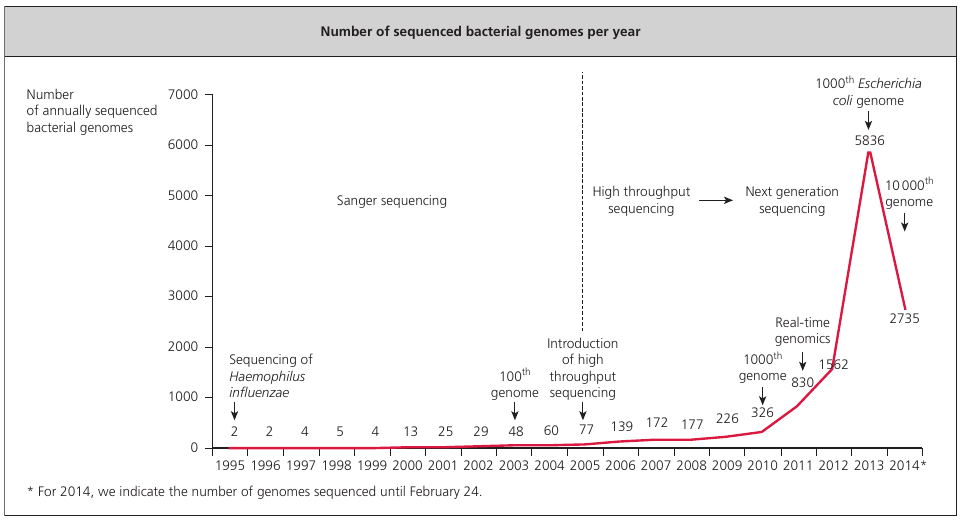
\includegraphics[width=0.9\linewidth]{images/sequencing_stats.png}
	\caption{Caption of fig. 1.}
	\label{fig:sequencing_stats}
\end{figure} 

With more than 49 000 bacterial genome sequences currently available,including those from all significant human pathogens, genomics has a significant impact on clinical microbiology and infectious diseases by enabling the development of improved diagnostic, genotyping, taxo-nomic, antibiotic and virulence marker detection tools as well as development of new culture media or vaccines. This chapter summarizes the current achievements in bacterial genomics relevant to medical microbiology.


\section{What is Genome Analysis?} 



